\chapter{Describing the design process}
\label{chap:design}
% Design: formules, inputs, outputs etc

%algemeen beamforming							(Niels)
%Beamformers provide an effective and versatile means of spatial filtering \cite{vanveen1988}. 
Beamformers are useful when distinguishing desired signals from noise and interference based on their locations \cite{himawan2011}. There are different beamforming algorithms with their own advantages and disadvantages. 

In this research, the delay-and-sum beamforming algorithm \cite{elko1996} and the MVDR algorithm \cite{habetsspeech2010} will be discussed. The DSB will be considered since this is a good baseline method to compare the other beamformer with. The MVDR has been chosen since the generalized sidelobe cancellar beamformer suffers from steering vector errors and the MVDR suppresses coherent noise well.


%The original MVDR is excessively sensitive to source location and microphone gains \citep{ba2007}. Microphone arrays are a common way to improve sound quality; the diversity in the received signals is exploited by setting different gains to each microphone, depending on the location of the source and on the auxiliary sources and noise. This is generally referred to as beamforming. There are different beamforming algorithms each with their own advantages and disadvantages. The delay-and-sum beamformer (DSB) is one of the earliest beamforming algorithms. It is a "fixed" beamformer, meaning that it only adapts to the locations of the microphones and the desired source. It delays and optionally weighs the microphone signals based on the distances and the speed of sound and the attenuation of the soundwave respectively bofore taking the average of the signals. The MVDR beamformer is one of the most widely used beamformers and can be used for both speech dereverberation and noise reduction.

%and a broadband region-based near-field beamforming algorithm \cite{martinez2015} that we refer to here as the ``Delft'' algorithm.

%In the scenario outlined in section {\ref{chap:introduction}} the dimensions of the microphone array are large with respect to the distance between the array and the source. Therefore we can assume that the sources of interest are mostly in the near-field region \cite{gaubitch2014}. In addition, the positioning of the microphones is arbitrary, but known. As such, the main focus for our implementation will be near-field beamforming with ad-hoc microphone arrays. In particular, we will research the benefits of compensating for the directivities of the microphones in the smartphones, as \cite{gaubitch2014} shows this having a positive effect on beamformer performance. To estimate the performance of our algorithms, the results will be evaluated using different intelligibility measures \cite{taal2010,rix2001}.

\section{Simulation}
\label{sec:des_simulation}

In this research, a simulation is used to simulate the effect of a reverberant room on the acoustic signals received at multiple microphones. This algorithm has been implemented in \matlab to simulate recording multiple audio sources in a room with multiple microphones. The simulation will be used to compare to the experimental results. The acoustic impulse response of a room characterizes the acoustics of that room. The convolution between the sound coming from the source and the impulse response results in the sound recorded by the microphones. The simulated microphones are omnidirectional, which means that the directivities of the microphones are not included in this simulation.

The parameters that can be set for this simulation are:

\begin{itemize}
\item Locations of the audio sources and the microphones. 
\item Size of the room.
\item Reflection coefficients.
\item SNR at which Gaussian white noise will be added.
\item Amount of random errors added to the microphone positions.
\item Reverberations on or off.
\end{itemize} 

Local stored audio files are expected as source files. The audio files will be trimmed down or zero padded to match the simulation time. Then the implemented algorithm calculates the impulse response of a room. The locations of the sources and the locations of the microphones and the size of the room will be used to calculate the impulse response between each source and each microphone. The impulse response is calculated using the image method \cite{allen1979}. This method mirrors the walls of a room and puts the sources in imaginary rooms next to the room in which the source and receiver are placed. This concept is illustrated in figure \ref{fig:image_method}. The standard image method has been modified to simulate received echo arrival time to estimate the intermicrophone phase \cite{peterson1986}.

\begin{figure} [h]
    \centering
       \includegraphics[page=2, scale = 1, clip=true, trim=10.5cm 23.3cm 4.5cm 1.5cm]{image_method.pdf} % l b r t
    \caption[Image method for simulating a rooms \cite{allen1979}]{Image method, "x" stands for an audio source and an "o" stands for a microphone. \cite{allen1979}}
    \label{fig:image_method}
\end{figure}

After calculating the impulse response of the room it is possible to determine the signal recorded by each microphone. The convolution of the source signals with the impulse responses result in an output signal for each microphone.

This is done by calculating the convolution between the impulse response of the room and the associated audio source. After this is done for each audio source and each microphone, white noise is added to make the simulation more realistic.

Having implemented this algorithm, the choice can be made to either record audio and apply the beamforming algorithm to that or use the simulation to create the input for the beamforming algorithm. The simulation calculates the acoustic impulse of the room which will be used to generate the sound recorded by the microphones. One of the impulse responses for a simulation without reverberations and one impulse response for a simulation with reverberations is plotted and can be found in figure \ref{fig:imp} and \ref{fig:impRev}.


\begin{figure}
	\centering  
	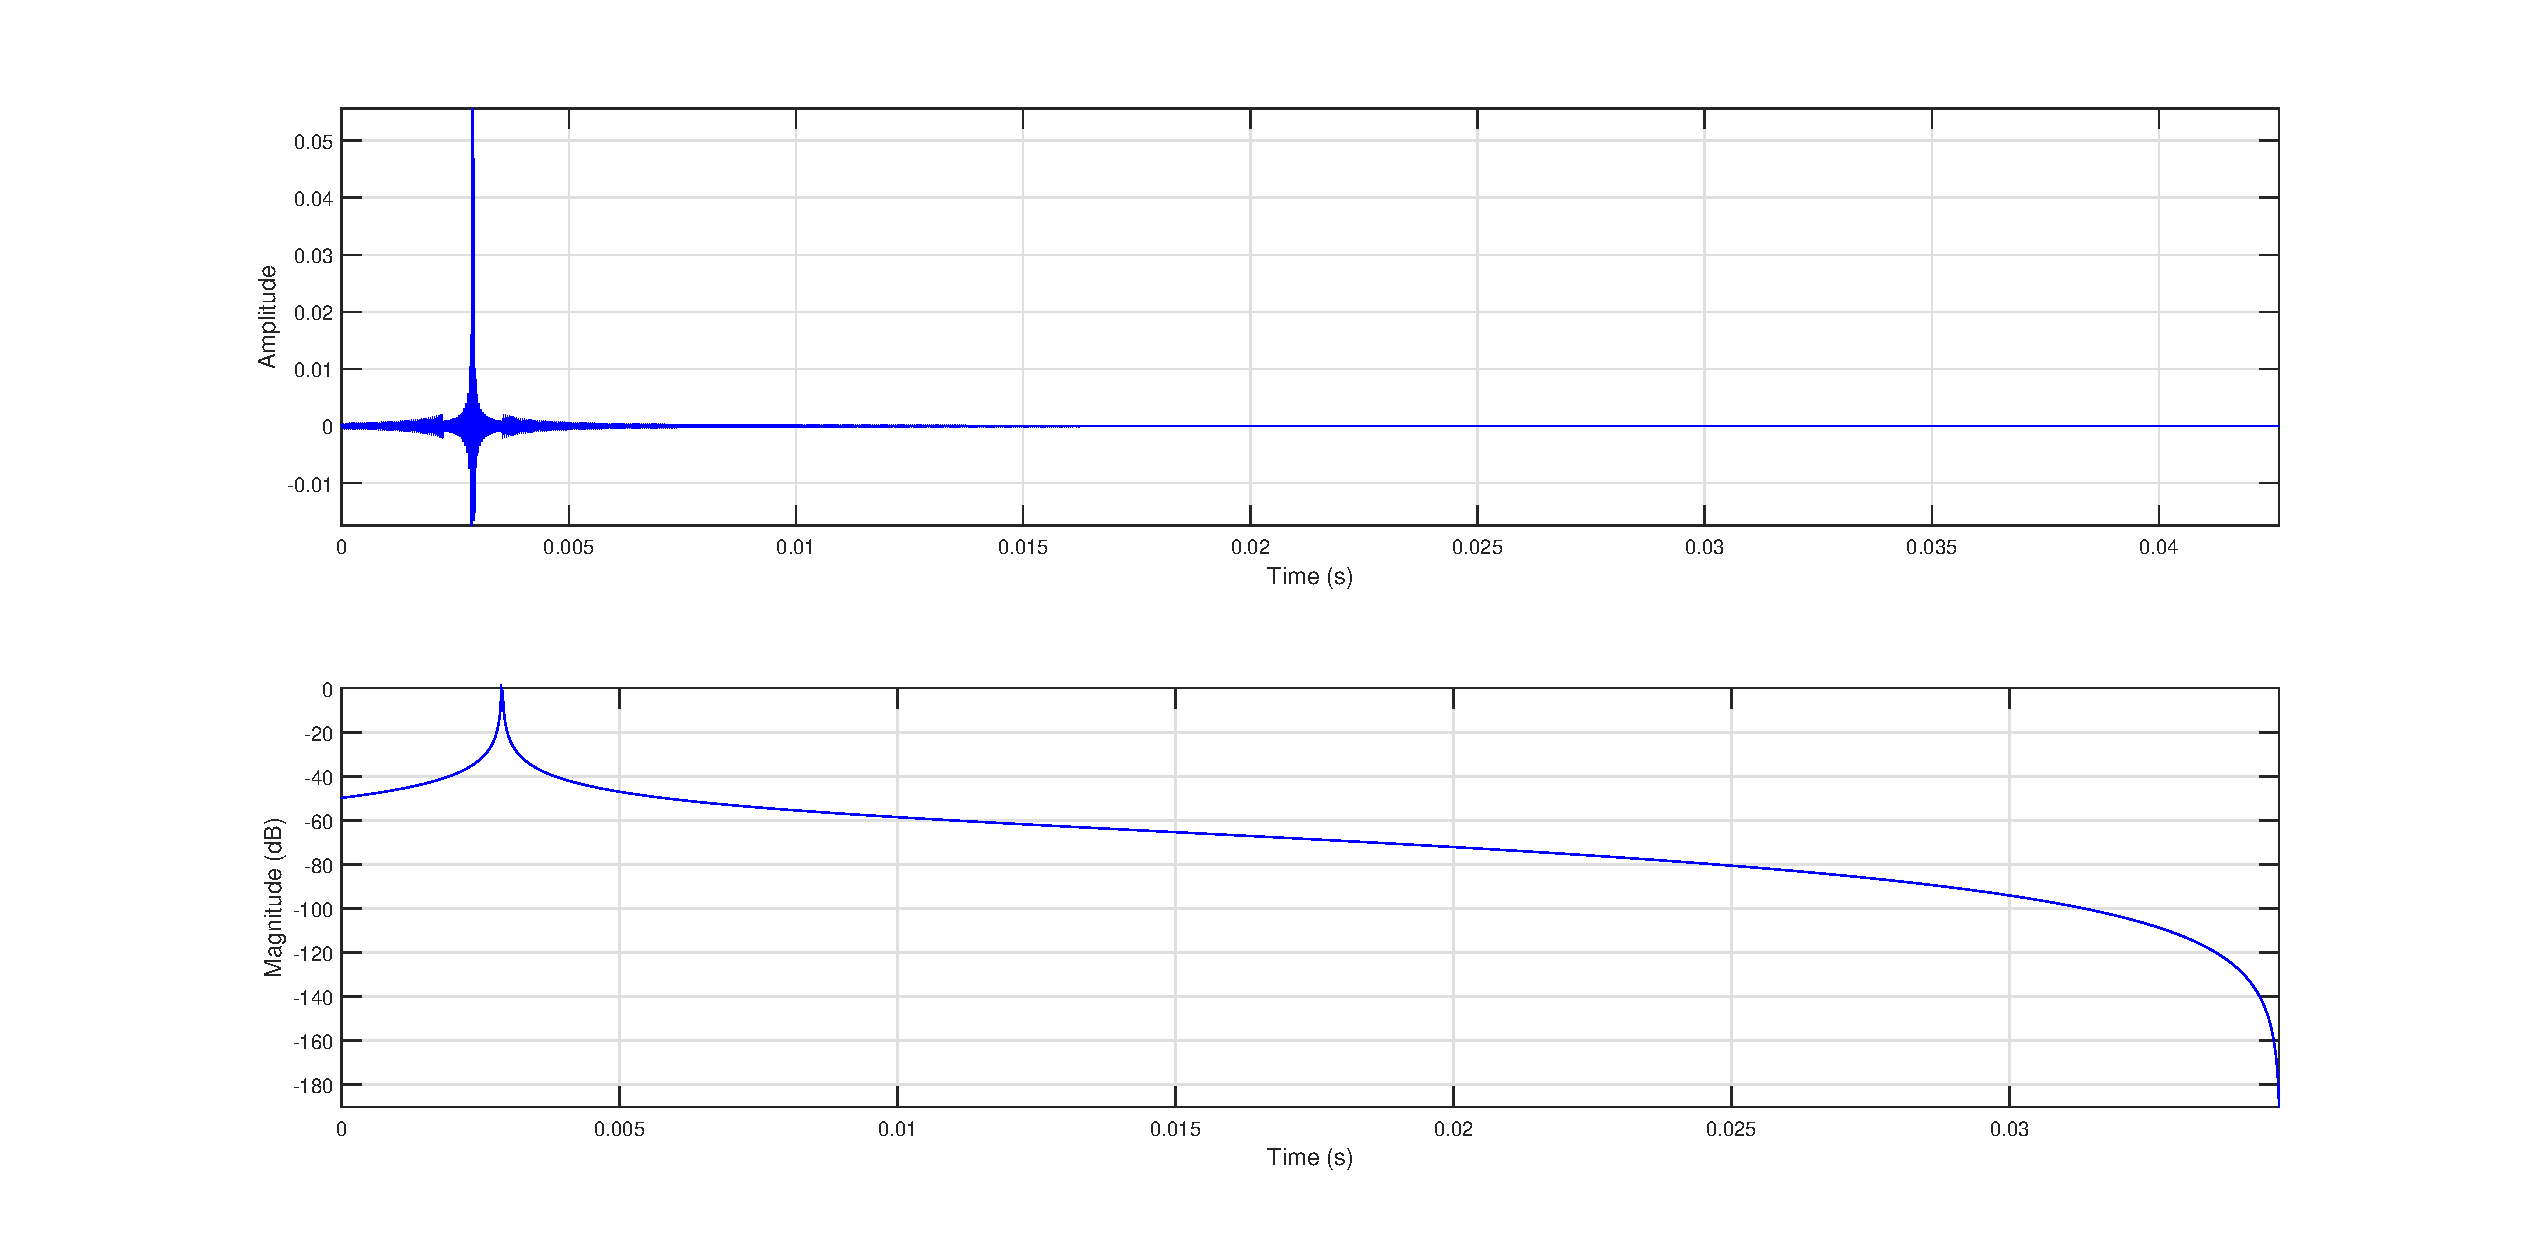
\includegraphics[width = 0.8\columnwidth, clip=true, trim= 0 1.1cm 0 0]{Screenshots_simulatie/Impulse_response/Simulatie_3}
	\caption[Simulated Impulse response without reverberations]{Simulated impulse response without reverberations in time-domain} 
	\label{fig:imp}
\end{figure}

\begin{figure} [h!]
	\centering  
	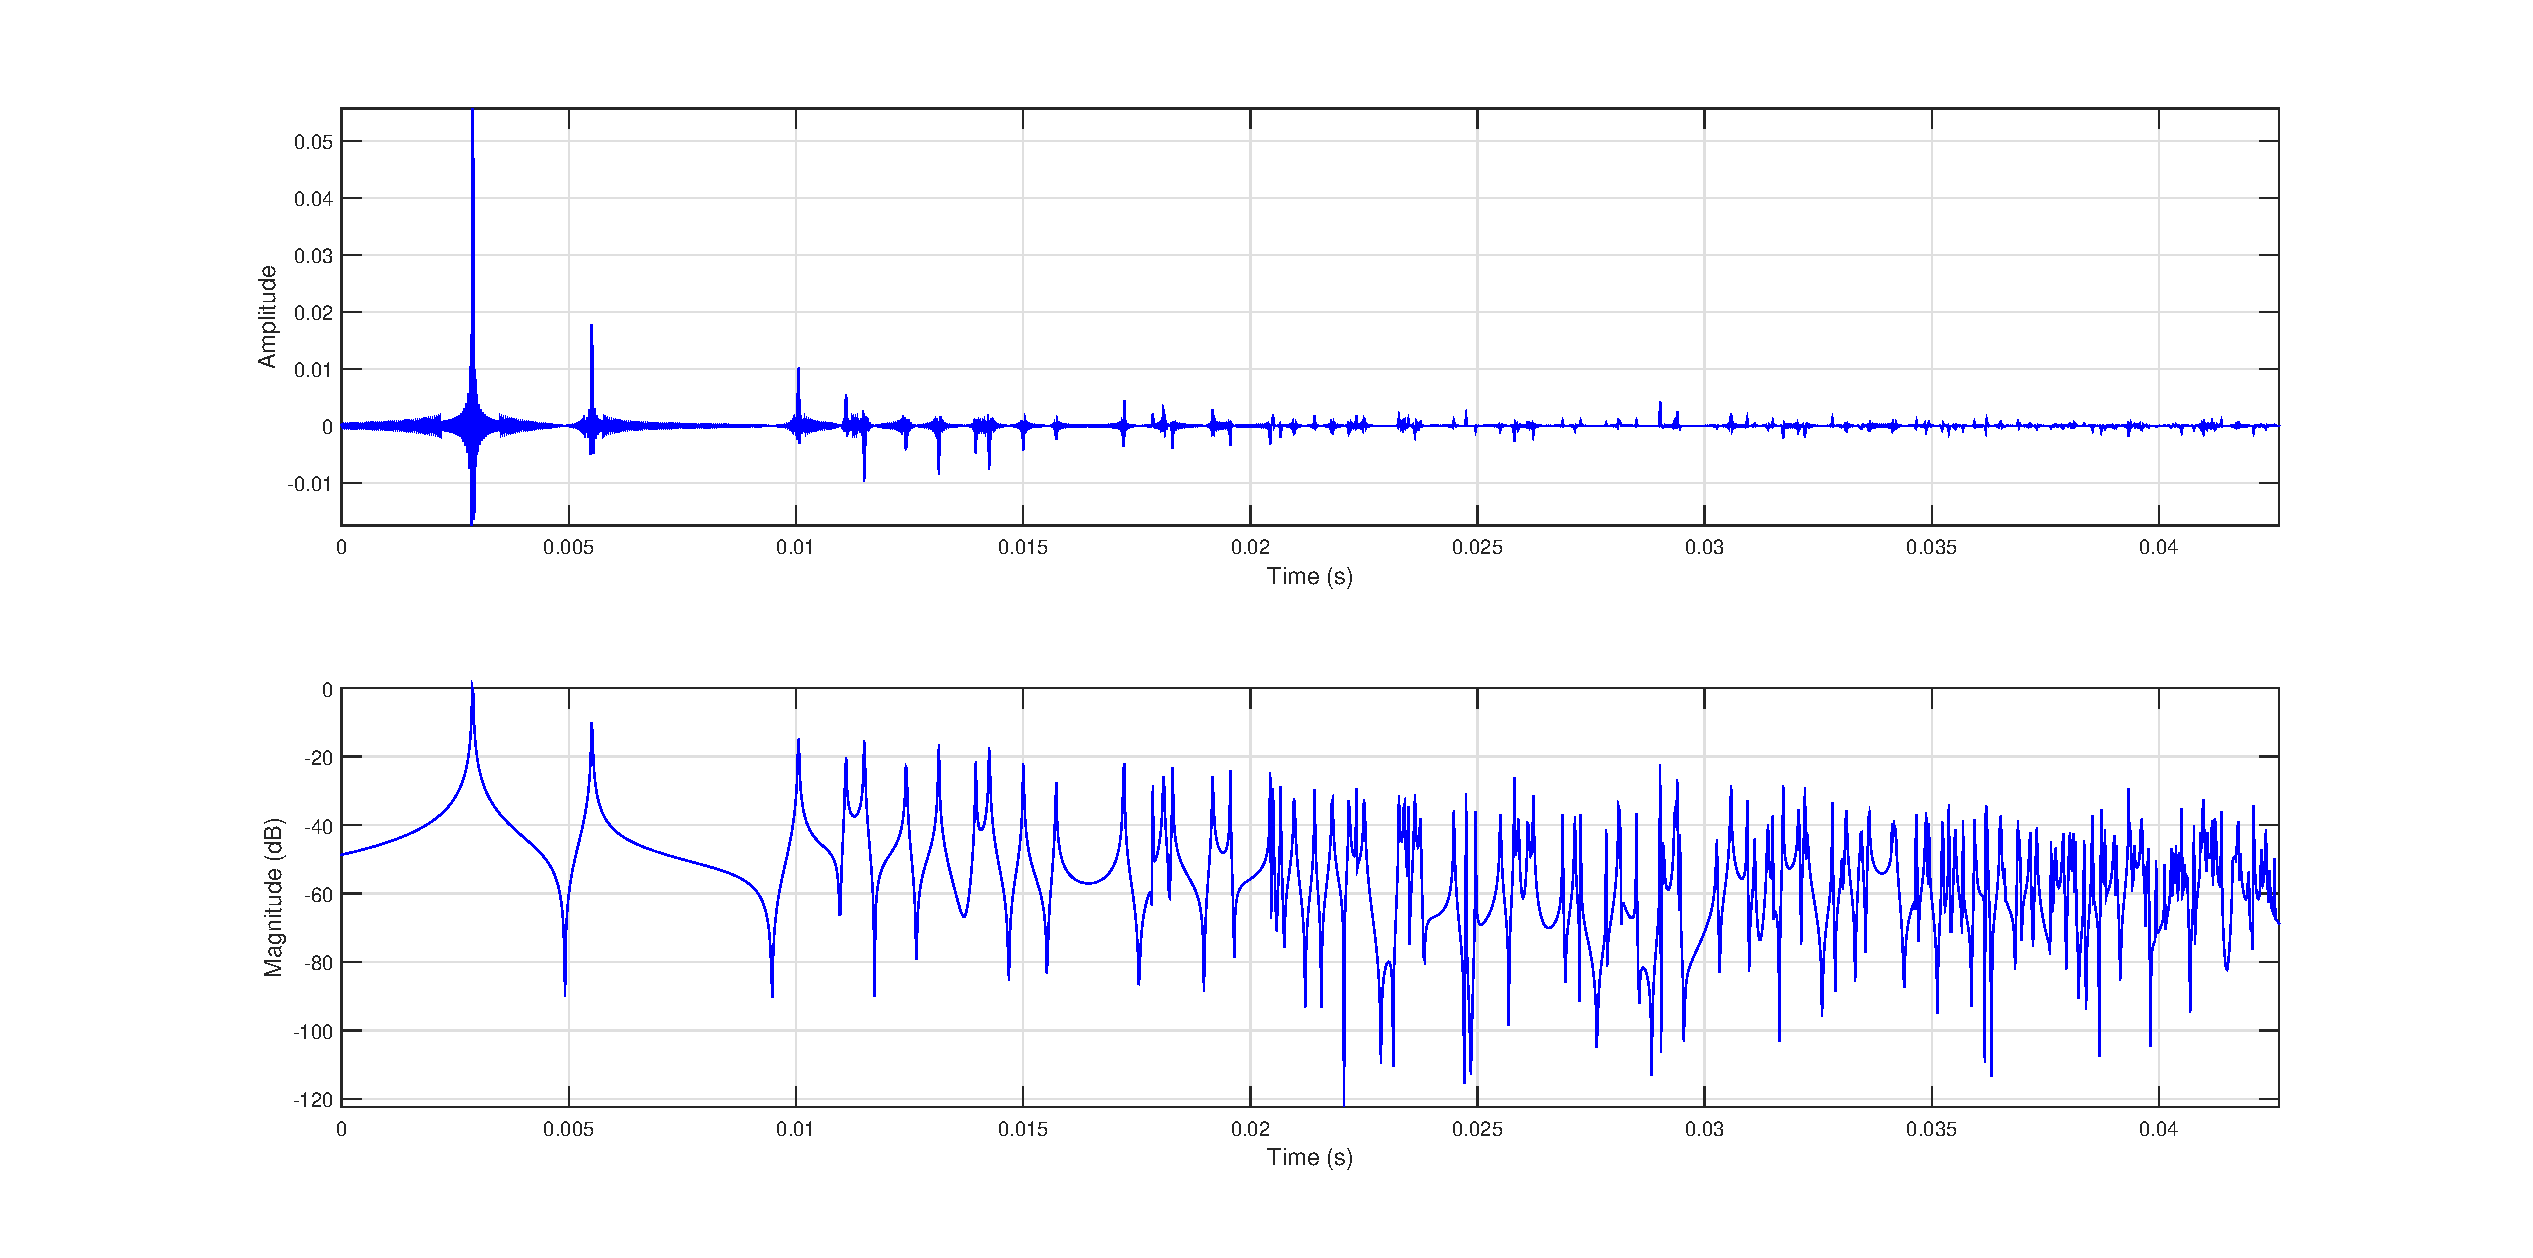
\includegraphics[width = 0.8\columnwidth, clip=true, trim= 0 1cm 0 0]{Screenshots_simulatie/Impulse_response/Simulatie_4}
	\caption[Simulated Impulse response with reverberations]{Simulated impulse response with reverberations in time-domain} 
	\label{fig:impRev}
\end{figure}

\section{Beamforming}
\label{sec:des_beamforming}
The technique called beamforming combines sensor array signals in some optimal manner such that the output approximates the desired source and suppresses the undesired noise/interferers. By choosing sensible weights a beamformer can perform spatial filtering with the goal of maximizing the intelligibility of the received signal.

The goal of beamforming is to estimate the desired signal $\hat{S}$ from equation \ref{eq:bf_est} as a linear combination of the data collected at the array. In other words, we would like to determine an $M \times 1$ vector weights $w(\omega)$ such that $\textbf{w}^{H}(\omega)\textbf{Y}(\omega)$ is a good estimate of $S(\omega)$.

The delay-and-sum beamformer (DSB) is one of the earliest beamforming algorithms. It is a "fixed" beamformer, meaning that it only adapts to the locations of the microphones and the desired source. The MVDR beamformer is one of the most widely used beamformers and can be used for both speech dereverberation and noise reduction.

%\nomenclature{$w$}{Weight in the frequency domain}

\subsection{Delay-and-sum Beamformer}
\label{sec:des_dsb}
%Erik
The delay-and-sum beamformer (DSB) first delays and weighs the microphone signals and then sums or averages the results for all the microphones. For the simple DSB the complex weights $\textbf{w}$ usually consists of only the delays. In near-field (Section \ref{sec:problem_near-field} applications the DSB may also perform inverse distance weighing in addition to delaying the signal to correct for attenuation losses. In the time domain the output $\overline{x}[n]$ can be written as \cite{naylor2010speech}:

\begin{equation}
\overline{x}[n] = \sum_{i=1}^{M} w_{i}x_{i}[n-\tau_{i}]
\end{equation}

\nomenclature{$\overline{x}(n)$}{Average estimated clean speech signal in the time domain}

%Delay-and-sum
If we take the discrete time Fourier transform and move the delay into the weight we get for the weights $\textbf{w} = [w_1,w_2,\dots,w_i,\dots,w_M]$: 

\begin{equation}
w_i(\omega) = \frac{1}{M} e^{-j\omega\tau_i}
\end{equation}
or with inverse distance weighing:
\begin{equation}
w_i(\omega) = \frac{1}{4\pi r_{i} M} e^{-j\omega\tau_i}
\end{equation}

with $M$ the number of microphones, $i \in \{1,2,\dots,M\}$, $w_{i}$ the weight applied to the $i^{th}$ microphone and $\tau_{i}$ the propagation delay in samples. This weight can be used to estimate the source signal described in equation \ref{eq:bf_est}. \newline
The best asset of the DSB is that the direct path components of the microphone signals will be coherent and therefore added constructively. The incoherent components, due to reverberation and noise, will be attenuated.

\subsection{Minimum variance distortionless response Beamformer}
\label{sec:des_mvdr}
%Erik
A general description of MVDR beamformers in room acoustics and the trade-off between speech dereverberation and noise reduction is described by Cohen et al.\cite{habetsspeech2010} and Habets et al. \cite{habetsroom2010}. The MVDR beamformer is derived by minimizing the energy of the observed signal, subject to the constraint that the signal in the desired look position remains undistorted \cite{vanveen1988}. It minimizes the variance of the noise component of $\textbf{w}^{H}\textbf{Y}$ from equation \ref{eq:bf_est}, subject to a constraint of gain 1 in the look direction \cite{ba2007}. The corresponding weight vector $\textbf{w}$ is the solution to the following optimization problem:

\begin{equation}
\hat{\textbf{w}} = \argmin_\textbf{w} \textbf{w}^H \Phi_\textbf{Y} \textbf{w} \quad\textrm{s.t.}\quad\textbf{w}^H\textbf{d} = 1
\end{equation}

\nomenclature{$\hat{\textbf{w}}$}{Vector of estimated complex weights}
\nomenclature{$\Phi$}{Covariance matrix of the microhone signals}

where $\Phi_\textbf{Y}$ is the covariance matrix of the observed signal\footnote{This is actually true for Minimum Power Distortionless Response (MPDR), for traditional MVDR the covariance matrix of the combined noise signals sould be used, e.g. the covariance matrix of the reflected paths and auxilary sources \cite{gannot2010}.}. $\Phi_\textbf{Y}$ is given by $\Phi_\textbf{Y} = E[\textbf{YY}^H]$, where $E[\bullet]$ denotes the expected value function. This optimization problem has an elegant closed-form solution published by Cox et al.\cite{cox1987}:

\begin{equation}
\label{eq:cox}
\hat{\textbf{w}} = \frac{\Phi_{\textbf{Y}}^{-1}\textbf{d}}{\textbf{d}^{H}\Phi_{\textbf{Y}}^{-1}\textbf{d}}
\end{equation}

The denominator of this equation contains a normalization factor which enforces the gain constraint in the look direction. The numerator contains the minimized energy information for MPDR, or minimized noise information for traditional MVDR, for the respective microphones.

\subsection{MVDR with Directivity}
\label{sec:des_mvdr_dir}
To illustrate how to include the microphone directivities in the algorithm a similar approach to Gaubitch et al. \cite{gaubitch2014} will be followed, which is outlined in this section. The theory of how to include directive (non-omnidirectional) microphones into the MVDR algorithm was briefly covered in section \ref{sec:observation}. The difference is not in the algorithm, but in the used impuls response. \newline
For omnidirectional microphones the signal received at each microphone ($Y_{i}$) consists of the following components:

\begin{equation}
Y_{i}(\omega) = S(\omega)H_{i}(\omega) + V_{i}(\omega)
\end{equation}

When the microphones are directive the signal is convolved with the microphone directivity $G(\omega, \theta, \phi)$. We end up with:

\begin{equation}
Y_{i}(\omega) = S(\omega)H_{i}(\omega)G_{i}(\omega, \theta, \phi) + V_{i}(\omega)
\end{equation}

The estimated source signal is again calculated by:
\begin{equation}
\hat{S}(\omega) = \textbf{w}^{H}(\omega)\textbf{Y}(\omega)
\end{equation}

with the weights estimate from equation \ref{eq:cox}.

\section{Assessing Beamforming Quality}
\label{sec:des_evaluation}
%Niels
Six measures are used to evaluate the performance of the beamformer. Speech intelligibility is evaluated by the objective intelligibility measures PESQ and STOI. The other measures that are used are the global and segmental SNR, the white noise gain and the array gain.

The PESQ and STOI algorithms both compare the original and processed signal. The chosen implementation of the PESQ is the ITU-T recommendation P.862 in 2002 \cite{itu2010}. A general overview of the PESQ, given by the ITU-T Recommendation P.862, is illustrated in figure \ref{fig:PESQ_overview}. First, the delays between the original and processed signal are calculated to align the signals in time. Based on the delays, PESQ compares the signals using a perceptual model. This perceptual model is done by transforming the signals to an representation that is analogous to the psychophysical representation of audio signals in the human auditory system. The final step of the PESQ algorithm is using a cognitive model to compute two error parameters, one without and one with an asymmetry factor \cite{rix2001}.  These parameters are combined to give an objective listening quality MOS. The output of the PESQ is a number in the range of $-0.5$ to $4.5$, where $-0.5$ is the lowest quality and $4.5$ is the highest quality.

\begin{figure}
    \centering
       \includegraphics[page=11, scale = 1, clip=true, trim=3.5cm 5.3cm 3.5cm 15.65cm]{PESQ.pdf} % l b r t
    \caption[General overview of the PESQ algorithm \cite{itu2010}]{Overview of the PESQ algorithm \cite{itu2010}}
    \label{fig:PESQ_overview}
\end{figure}

The other intelligibility measure used to determine the performance of the beamformer was STOI. The used algorithm was proposed and implemented by taal et al. \cite{taal2010,taal2011}.

The SNR is calculated by dividing the power of the signal by the power of the noise by the following equation:\cite{kondo2012}

\begin{equation}
\text{SNR} = 10log_{10} \frac{\sum_{n=1}^{N} x^2(n)}{\sum_{n=1}^{N} \{x(n) - \hat{x}(n)\}}
\end{equation}

Where x(n) is the clean speech signal, $\hat{x}(n)$ is the distorted speech and N is the number of samples.

\nomenclature{$x(n)$}{Clean speech signal in the time domain}
\nomenclature{$\hat{x}(n)$}{Distorted speech signal in the time domain}
\nomenclature{$N$}{Number of samples}

The classical SNR is not well related to to the speech quality and therefore the segmental SNR ($SNR_{seg}$) will also be calculated. $SNR_{seg}$ calculates the SNR in short frames and then takes the average of the frames. 

\begin{equation}
SNR_{seg} = \frac{10}{K} \sum_{k=0}^{K-1} log_{10} \frac{\sum_{n=L_{f}k}^{L_{f}k+L_{f}-1} x^2(n)}{\sum_{n=L_{f}k}^{L_{f}k+L_{f}-1} \{x(n)-\hat{x}(n)\}^2}
\end{equation}
Were $L_{f}$ is the frame length and $K$ the number of frames in the signal. By determining the energy in each frame it is possible to limit This calculation to the frames in which speech is active. The audio frames without speech will be discarded.

\nomenclature{$\text{SNR}_\text{seg}$}{Segmental signal-to-noise ratio [dB]}
\nomenclature{$L_{f}$}{Frame length of the segmental signal-to-noise ratio [s]}

\section{Realtime Beamforming Toolbox}
\label{sec:des_gui}
To make it easier to repeat the beamforming experiments a \matlab toolbox has been developed. The approach of this toolbox is based on the Model-view-controller-model (MVC). Beamforming scripts (of which there are many available on the internet) can be coded into a standard processing unit to use them in real time. Changes to individual algorithms may have to be made to make them run in realtime and the input variables may have to be relabeled. \newline
In this section the implementation of the system is described. Figure \ref{fig:UI_schematic} shows a flowchart of the system. The green blocks (on the left side) are possible inputs. The orange blocks show inputs that have to be set from the UI. The rightmost blocks are the processing algorithms.

\begin{figure}
    \centering
       \includegraphics[scale = 0.6, clip = true]{images/beamforming_UI_schemetic.png} % l b r t
    \caption[Beamforming Toolbox flowchart]{Beamforming Toolbox flowchart.}
    \label{fig:UI_schematic}
\end{figure}

%\begin{figure} [b]
%    \centering
%       \includegraphics[scale = 1, clip = true, trim=10.5cm 23.3cm 4.5cm 1.5cm]{images/beamforming UI schemetic.pdf} % l b r t
%    \caption[Beamforming UI flowchart]{Beamforming UI flowchart.}
%    \label{fig:UI_schematic}
%\end{figure}

\subsection{Data Acquisition}
\label{sec:des_aqc}
Data inputs can be audio files, computer audio input channels, smartphones that run the Android app or multiple microphone locations can be simulated using different simulation options. Data from files can be loaded at once. The smartphones and computer microphones stream the data in small frames and call an update function when there is new data available. All inputs can be sampled at or resampled to other sample rates, but standard $48000 Hz$ is used. The data is usually sampled with a resolution of $16$ bits per sample, but as many steps in the computation require the data to be in double precision the data is stored in memory in double precision.


%Design process of Graphical user interface
%Erik

\subsection{Buffer}
\label{sec:des_buffer}
A fast data buffer has been implemented that serves as the core of the toolbox. All algorithms access the data so there need not be multiple copies of large data variables in memory. All of the used algorithms process the data in frames and write the processed data back to the buffer. This, in combination with proper memory allocation makes the toolbox run fast on large data sets as well as on smaller ones, as long as there is enough memory available. The buffer was tested with at most an hour of streaming audio from three smartphones, which resulted in about $3 GB$ of memory use. \newline
The properties of the data that are stored in the buffer are:
\begin{itemize}
\item Sample rate, $48000 Hz$
\item Bits per Sample, $16$
\item Number of Channels
\item Channel Name, reserved names are: $^*Mic, ^*Source, ^*Noise, ^*Beamformer$
\item Locations, $[x,y,z,az,el,up]$
\item Current Sample, stores the index of the last sample in the buffer for each channel
\item Total Samples
\item Audio Data, matrix of size Number-of-Channels-by-Total-Samples
\end{itemize}

The locations are stored as vectors with in the first three entries the position in 3D, followed by the azimuth and elevation, and finally a boolean value for up or downward facing of the smartphone (screen). The latter three are only used for directional microphones and the last one is only used for smartphones. 

\subsection{Synchronized Recording}
\label{sec:des_sync}
Because the channels use multiple hardware devices the channels do not start the recording at the same time. A synchronized recording method has been developed to overcome this problem, similar to the method proposed by Bosma and Smeding \cite{BAP:RoySjoerd}.
When synchronized recording is started the computer adds a Maximum Length Sequence (MLS) at the beginning of the source recording. The MLS pulse has many nice properties but the most interesting one here is that the autocorrelation approaches a Kronecker delta \cite{hee2003impulse}. Sufficient time for the synchronization to finish is also added before the source signal starts. The correlation between the MLS pulse in the source channel and the recorded MLS pulse is calculated and the highest value corresponds to the Kronecker delta, at the time offset between the signals.
the time offset. This method is used on all the channels in the buffer to calculate the delay between when the first sample was taken and when the MLS pulse was received. \newline
The TDOAs of all channels, calculated from locations inputted by the user, are substracted from this delay to force the TDOA of the channels to correspond to the locations. \newline
A delayChannel method then shifts the samples in the buffer and the delays are added to the current sample value of the channel to ensure samples arriving in the future are lined up in time.

\subsection{Processing Unit}
\label{sec:des_processing}
Realtime processing of data which is arriving at irregular intervals and in irregular order has been made implicit by having the buffer store current sample values for each channel. The processing units check whether the current sample value of the listening channel plus the size of their frames is larger than the minimum of the current samples of each of the connected input channels. It will then loop over all available frames and put the processed data in their output channel in the buffer. This makes processing large files from the disk go as fast as the computations will allow, and processing streaming data go in realtime for beamformers which don't have too large complexity. The MVDR beamformer complexity increases hugely with the number of input channels. For our purposes realtime means that the incoming and outgoing audiosignals, the beamformed signals and the $SNR$ and $SNR_{seg}$ can be plotted on screen with less than a second delay.

\begin{figure} [h]
    \centering
       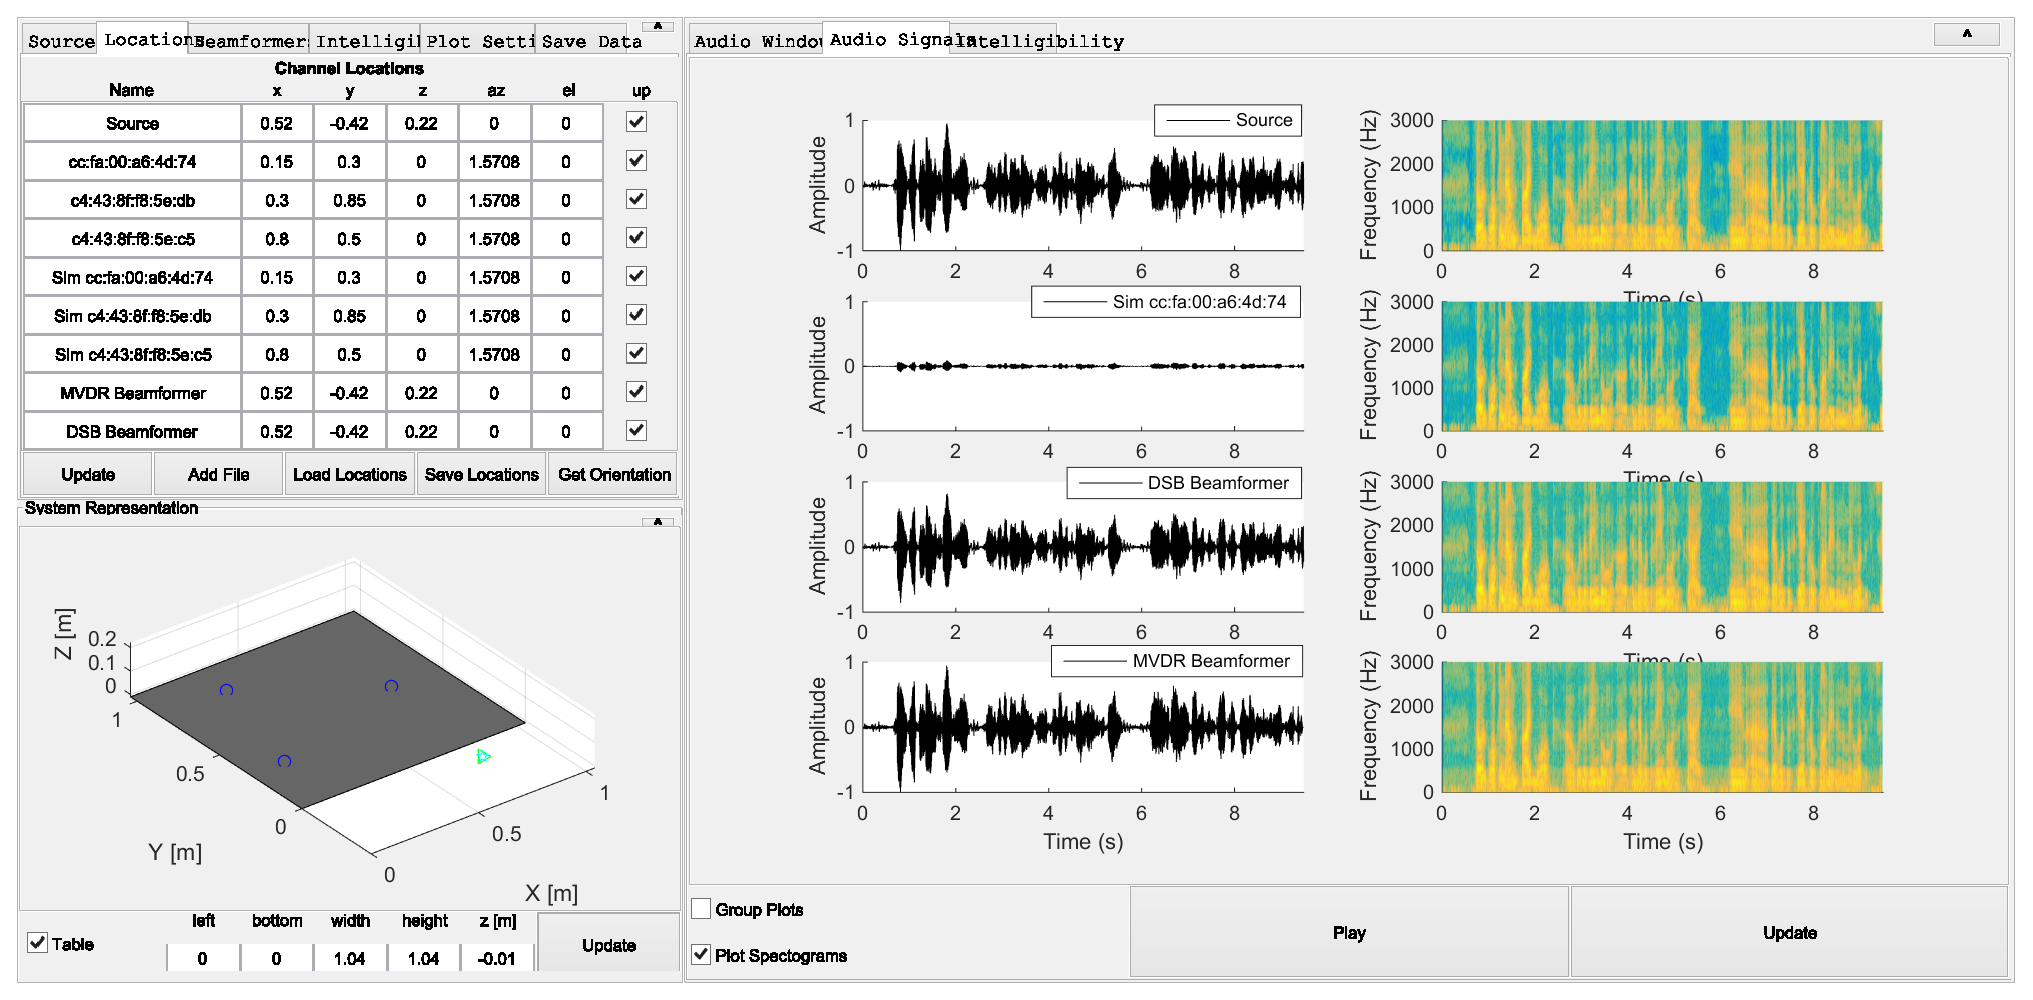
\includegraphics[width = \columnwidth]{GUI_screenshot.eps} % l b r t
    \caption[User interface implemented in \matlab]{Matlab Realtime Beamforming Toolbox GUI}
    \label{fig:GUI}
\end{figure}

\subsection{User Interface (UI)}
\label{sec:des_realtime}
The UI has been build with a modular design. Every UI panel can run individually, or they can be connected with a main object that has multiple UI panels. There is a panel where frames from the buffer can be plotted in realtime and one where the whole channel can be plotted. These can also be used to easily playback (part of) the data and to plot the frequency spectrum against time. There is a panel where the intelligibility metric outputs are shown. Each of the inputs has its own panel with buttons to start or stop streaming or several others. There is a panel which can be used to save data to multiple audio formats, with the locations stored in the meta-data of the audio file, or as \matlab .mat files, with all relevant labels saved. Each of the beamformers has a panel to change their parameters and to enable them, or to process data at once. The intelligibility metrics have a similar panel and a separate panel where the metrics are shown, and the output of the $SNR$ algorithm is plotted against time. There is a standard selector panel which is used in multiple places to connect inputs to processing units. All the locations can be entered in the locations panel. Lastly there is a system representation tab which plots the locations of the channels in the buffer on an axis and can also draw a tabletop surface. This makes it easy to compare modeled scenario with the real scenario.
